%!TEX root = report.tex
\subsection{Arrival}
\par This endpoint serves as a wrapper for the Tfl Live Bus API endpoint. Given a set of \acrfull{gps} coordinates and the radius of circle, this API endpoint returns the arrival times of buses arriving at stops within the circle.

\subsubsection{Query URL \& Parameters}
\par The base URL for this endpoint is \url{http://delay.doc.ic.ac.uk:5000/arrivals/?}.

\par The required parameters include the latitude and the longitue of the \acrshort{gps} coordinates, and the radius in meters.

\par An example query URL would be \url{http://delay.doc.ic.ac.uk:5000/arrivals/?latitude=51.495171603309615&longitude=-0.1883983612060547&radius=100}.

\subsubsection{Result Format}
\par The query result is a list of bus stops within the circle. Each bus stop entry has basic information about the stop, and a list of the buses arriving at the stop in the next 30 minutes, grouped by the bus routes. Within each route, the \textbf{estimatedTimeInSeconds} shows the arrival times of the buses arriving at the given stop. See Figure \ref{fig:arrival_api} for example response.


\begin{figure}
\centering
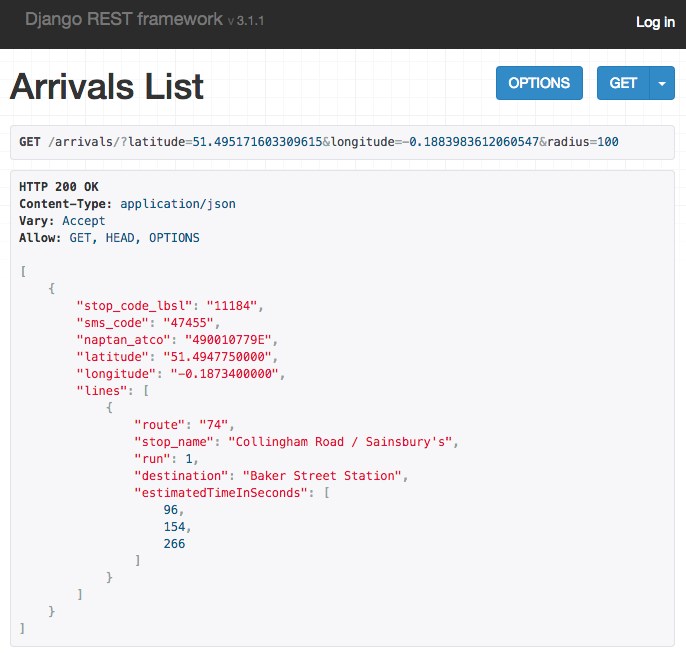
\includegraphics[width=\textwidth]{figures/arrival_api.png}
\caption{\label{fig:arrival_api} Sample Response for Arrivals API}
\end{figure}

\section{Summary of Data Service}
Building these three API endpoints helped us meet our first objective by supplying data on bus travel time predictions. We evaluated the accuracy and performance in Chapter \ref{ch:evaluation}.
